\documentclass[lang=cn,a4paper,newtx,bibend=bibtex]{elegantpaper}
\usepackage{env}
\title{Problems of Chapter 10.3.1-10.3.3}
\author{张志心 \ 计科2106}
\date{\zhdate{2024/04/08}}
\usepackage{env}
\pgfplotsset{compat=1.17}
\addbibresource[location=local]{reference.bib}
\begin{document}
\maketitle

\begin{prob}[Exercise 10.99]
  Compute the first five coefficients $C_j$'s 
  of the trapezoidal rule and the midpoint rule from
  Examples 10.85 and 10.87.
\end{prob}

\begin{solution}~~\\
\begin{enumerate}[(1)]
  \item Trapezoidal rule:
        \[
           \uB^{n+1} = \uB^n + \frac{k}2 \left(f(\uB^n, t_n) + f(\uB^{n+1}, t_{n+1})\right),
           s = 1, \alpha = \{-1, 1\}, \beta = \{\frac12, \frac12\}.
        \]
        $C_0 = \alpha_0 + \alpha_1 = 0, \quad C_1 = -\beta_0 + \alpha_1 - \beta_1 = 0, \quad 
        C_2 = \frac12 \alpha_1 - \beta_1 = 0$,\\
        $C_3 = \frac16 \alpha_1 - \frac12 \beta_1 = - \frac1{12}, \quad
        C_4 = \frac{1}{24} \alpha_1 - \frac16 \beta_1 = - \frac1{24}$.
  \item Midpoint rule:
        \[
          \uB^{n+1} = \uB^{n-1} + 2k f(\uB^{n}, t_n),s= 2, \alpha = \{-1, 0, 1\}, \beta = \{0, 2, 0\}.
        \]
        $C_0 = \alpha_0 + \alpha_1 + \alpha_2 = 0, \quad C_1 = -\beta_0 + \alpha_1 - \beta_1 + 2\alpha_2 = 0,$\\
        $C_2 = \frac12 \alpha_1 - \beta_1 + 2\alpha_2 = 0, \quad C_3 = \frac16 \alpha_1 - \frac12 \beta_1 + \frac43 \alpha_2 = \frac13$,\\
        $C_4 = \frac1{24}\alpha_1 - \frac16 \beta_1 + \frac23\alpha_2 = \frac13$.
\end{enumerate}
\end{solution}

\begin{prob}[Exercise 10.101]
  Express conditions of $\| \mathcal{L} \uB (t_n)\| = O(k^3)$
  using characteristic polynomials.
\end{prob}

\begin{solution}
  $\| \mathcal{L} \uB (t_n)\| = O(k^3)$ 要求 $C_0 = C_1 = C_2 = 0$,
  即
  \equ{
      C_0 &= \sum_{j = 0}^s \alpha_j = \rho(1) = 0, \\
      C_1 &= \sum_{j = 0}^s j \alpha_j - \sum_{j = 0}^s \beta_j = \rho'(1) - \sigma(1) = 0, \\
      C_2 &= \sum_{j = 0}^s \frac{j^2}2 \alpha_j - \sum_{j = 0}^s j \beta_j \\
          &= \frac12 \sum_{j = 0}^s j(j-1)\alpha_j + \frac12 \sum_{j=0}^s j\alpha_j - \sum_{j=0}^s j\beta_j \\
          &= \frac12 \rho''(1) + \frac12 \rho'(1) - \sigma'(1) = 0
  }
\end{solution}

\begin{prob}[Exercise 10.102]
  Derive coefficients of LMMs shown below
  by the method of undetermined coefficients and a programming 
  language with symbolic computation such as Matlab.
\end{prob}

\begin{solution}
\begin{enumerate}[(1)]
\item Adams-Bashforth formulas: $\alpha_s  = 1, \alpha_{s-1} = -1, \alpha_{s-2} = \dots = \alpha_0 = 0$,
\begin{figure}[H]
  \centering
  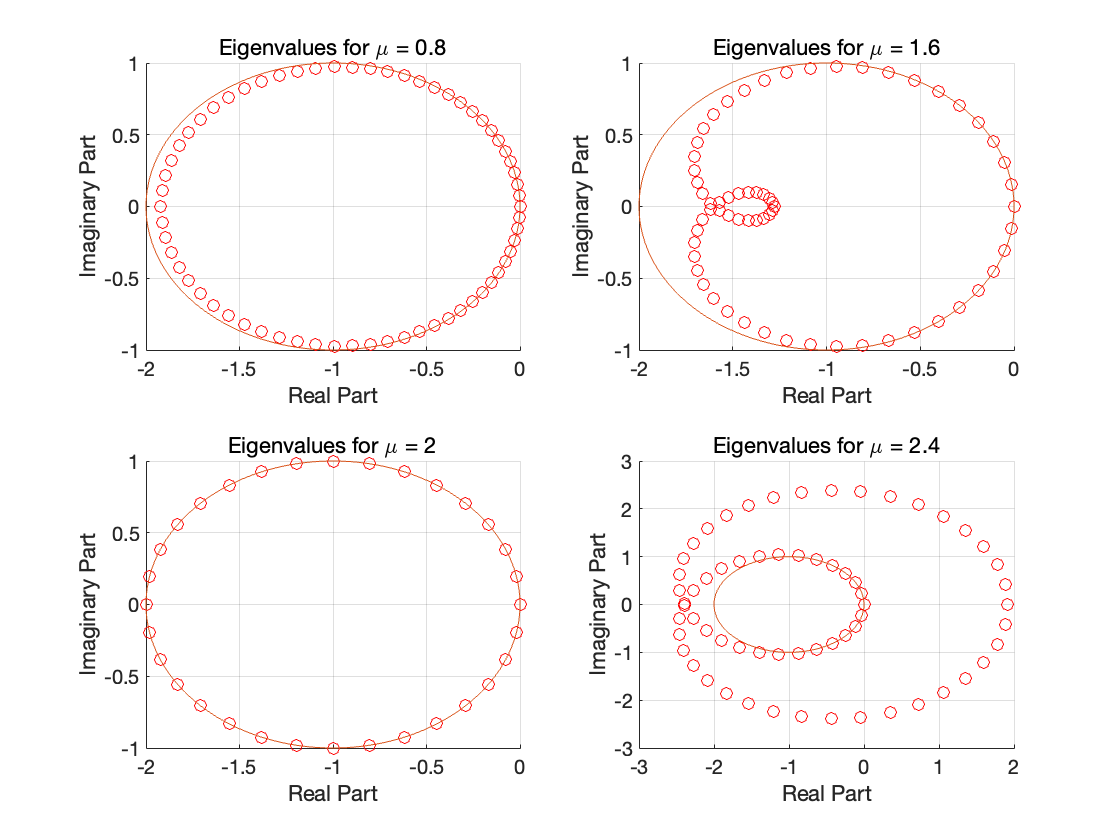
\includegraphics[width=0.5\textwidth]{1.png}
\end{figure}
\begin{itemize}
\item
$s = 1, p = 1, C_0 = C_1 = 0 \Rightarrow \alpha_1 - \beta_0 = 0 \Rightarrow \beta_0 = 1$.
\item 
$s = 2, p = 2, C_0 = C_1 = C_2 = 0 \Rightarrow 
\begin{cases}
  (\alpha_1 + 2 \alpha_2) - (\beta_0 + \beta_1) = 0 \\
  (\frac12 \alpha_1 + 2 \alpha_2) - \beta_1 = 0
\end{cases}
$\\$
\Rightarrow \begin{bmatrix} 1 & 1 \\ 1 & 0 \end{bmatrix}
\MAT{\beta_1 \\ \beta_0} = \MAT{1 \\ \frac32}
\Rightarrow \MAT{\beta_1 \\ \beta_0} = \MAT{\frac32 \\ - \frac12}.
$
\item 
$s = 3, p = 3, C_0 = C_1 = C_2 = C_3 = 0 \Rightarrow
\Cases{
  (2 \alpha_2 + 3 \alpha_3) - (\beta_0 + \beta_1 + \beta_2) = 0 \\
  (2 \alpha_2 + \frac92 \alpha_3) - (\beta_1 + 2 \beta_2) = 0 \\
  (\frac43 \alpha_2 + \frac92 \alpha_3) - (\frac12 \beta_1 + 2 \beta_2) = 0
}.
$\\
$
\Rightarrow 
\MAT{1 & 1 & 1 \\ 2 & 1 & 0 \\ 2 & \frac12 & 0}
\MAT{\beta_2 \\ \beta_1 \\ \beta_0} = 
\MAT{ 1 \\ \frac52 \\ \frac{19}6 }\Rightarrow
\MAT{\beta_2 \\ \beta_1 \\ \beta_0} = 
\MAT{ \frac{23}{12} \\ - \frac{16}{12} \\ \frac{5}{12}}.
$
\item
$s = 4, p = 4, C_0 = C_1 = C_2 = C_3 = C_4 = 0
\Rightarrow
\Cases{
  (3\alpha_3 + 4\alpha_4) - (\beta_0 + \beta_1 + \beta_2 + \beta_3) = 0 \\
  (\frac92\alpha_3 + 8\alpha_4) - (\beta_1 + 2\beta_2 + 3\beta_3) = 0 \\
  (\frac92\alpha_3 + \frac{32}3 \alpha_4) - (\frac12\beta_1 + 2\beta_2 + \frac92\beta_3) = 0 \\
  (\frac{27}8 \alpha_3 + \frac{32}{3}\alpha_4) - (\frac16 \beta_1 + \frac43 \beta_2 + \frac92 \beta_3) = 0
}$\\
$
\Rightarrow
\MAT{1 & 1 & 1 & 1 \\ 3 & 2 & 1 & \\ \frac92 & 2 & \frac12 & 0 \\ \frac92 & \frac43 & \frac16 & 0}
\MAT{\beta_3 \\ \beta_2 \\ \beta_1 \\ \beta_0} = 
\MAT{1 \\ \frac72 \\ \frac{37}6 \\ \frac{175}{24}} 
\Rightarrow \MAT{\beta_3 \\ \beta_2 \\ \beta_1 \\ \beta_0} = 
\MAT{\frac{55}{24} \\ - \frac{59}{24} \\ \frac{37}{24} \\ -\frac{9}{24}}.
$
\end{itemize}
\newpage
\item Adams-Moulton formulas: $\alpha_s = 1, \alpha_{s-1} = -1, \alpha_{s-2} = \dots = \alpha_0 = 0$,
\begin{figure}[H]
  \centering
  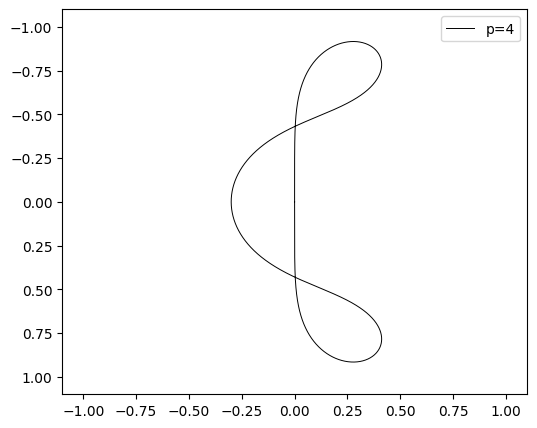
\includegraphics[width=0.5\textwidth]{2.png}
\end{figure}
\begin{itemize}
\item 
$s = 1, p = 1, C_0 = C_1 = 0 \Rightarrow \alpha_1 - \beta_1 = 0 \Rightarrow \beta_1 = 1$.
\item 
$s = 1, p = 2, C_0 = C_1 = C_2 = 0 \Rightarrow 
\Cases{
  - (\beta_0 + \beta_1) = 0 \\
  \frac12 \alpha_1 - \beta_1 = 0
}
$ \\
$
\Rightarrow
\MAT{1 & 1 & \\ 1 & 0}\MAT{\beta_1 \\ \beta_0} = \MAT{1 \\ \frac12}
\Rightarrow \MAT{\beta_1 \\ \beta_0} = \MAT{\frac12 \\ \frac12}.
$
\item
$s = 2, p = 3, C_0 = C_1 = C_2 = C_3 = 0 \Rightarrow
\Cases{
  (\alpha_1 + 2 \alpha_2) - (\beta_0 + \beta_1 + \beta_2) = 0 \\
  (\frac12 \alpha_1 + 2 \alpha_2) - (\beta_1 + 2\beta_2) = 0 \\
  (\frac16j \alpha_1 + \frac43 \alpha_2) - (\frac12 \beta_1 + 2 \beta_2) = 0
}$\\
$
\Rightarrow
\MAT{1 & 1 & 1 \\ 2 & 1 & 0 \\ 2 & \frac12 & 0}\MAT{\beta_2 \\ \beta_1 \\ \beta_0}
= \MAT{1 \\ \frac32 \\ \frac76} \Rightarrow \MAT{\beta_2 \\ \beta_1 \\ \beta_0}
= \MAT{\frac5{12} \\ \frac{8}{12} \\ -\frac1{12}}.
$
\item
$s = 3, p = 4, C_0 = C_1 = C_2 = C_3 = C_4 = 0 \Rightarrow
\Cases{
  (2 \alpha_2 + 3 \alpha_3) - (\beta_0 + \beta_1 + \beta_2 + \beta_3) = 0\\
  (2 \alpha_2 + \frac92 \alpha_3) - (\beta_1 + 2\beta_2 + 3 \alpha_3) = 0 \\
  (\frac43 \alpha_2 + \frac92 \alpha_3) - (\frac12 \beta_1 + 2 \beta_2 + \frac92 \beta_3) = 0\\
  (\frac23 \alpha_2 + \frac{27}{8} \alpha_3) - (\frac16 \beta_1 + \frac43 \beta_2 + \frac92 \beta_3) = 0
}
$\\
$
\Rightarrow
\MAT{1 & 1 & 1 & 1 \\ 3 & 2 & 1 & \\ \frac92 & 2 & \frac12 & 0 \\ \frac92 & \frac43 & \frac16 & 0}
\MAT{\beta_3 \\ \beta_2 \\ \beta_1 \\ \beta_0} = 
\MAT{1 \\ \frac52 \\ \frac{19}6 \\ \frac{65}{24}} 
\Rightarrow \MAT{\beta_3 \\ \beta_2 \\ \beta_1 \\ \beta_0} = 
\MAT{\frac{9}{24} \\ - \frac{19}{24} \\ -\frac{5}{24} \\ \frac{1}{24}}.
$
\item
$s = 4, p = 5, C_0 = C_1 = C_2 = C_3 = C_4 = C_5 = 0
\Rightarrow
\Cases{
  (3\alpha_3 + 4\alpha_4) - (\beta_0 + \beta_1 + \beta_2 + \beta_3 + \beta_4) = 0 \\
  (\frac92 \alpha_3 + 8\alpha_4) - (\beta_1 + 2\beta_2 + 3\beta_3 + 4\beta_4) = 0 \\
  (\frac{29}2 \alpha_3 + \frac{32}3 \alpha_4) - (\frac12 \beta_1 + 2 \beta_2 + \frac92 \beta_3 + 8 \beta_4) = 0\\
  (\frac{27}8 \alpha_3 + \frac{32}3 \alpha_4) - (\frac16 \beta_1 + \frac43 \beta_2 + \frac92 \beta_3 + 8 \beta_4) = 0 \\
  (\frac{81}40 \alpha_3 + \frac{128}{15} \alpha_4) - (\frac1{24} \beta_1 + \frac32 \beta_2 + \frac{27}8 \beta_3 + \frac{32}3 \beta_4) = 0
}
$ \\
$
\Rightarrow
\MAT{1 & 1 & 1 & 1 & 1 \\
     4 & 3 & 2 & 1 & 0 \\
     8 & \frac92 & 2 & \frac12 & 0 \\
     \frac{32}3 & \frac92 & \frac43 & \frac16 & 0 \\
     \frac{32}3 & \frac{27}8 & \frac32 & \frac1{24} & 0}
\MAT{\beta_4 \\ \beta_3 \\ \beta_2 \\ \beta_1 \\ \beta_0} 
= \MAT{1 \\ \frac72 \\ \frac{37}6 \\ \frac{175}{24} \\ \frac{781}{120}}
\Rightarrow
\MAT{\beta_4 \\ \beta_3 \\ \beta_2 \\ \beta_1 \\ \beta_0} 
= \MAT{\frac{251}{720} \\ \frac{646}{720} \\ -\frac{264}{720} \\ \frac{106}{720} \\ -\frac{19}{720}}
$
\end{itemize}
\item Backward differentiation formulas:$\beta_{s-1} = \dots = \beta_0 = 0$,指定 $\alpha_s = 1$,
\begin{figure}[H]
  \centering
  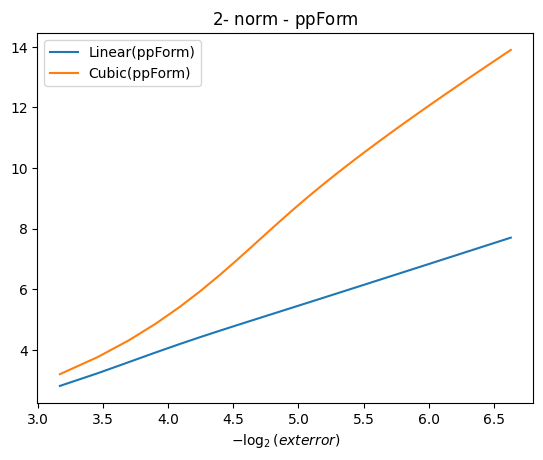
\includegraphics[width=0.5\textwidth]{3.png}
\end{figure}
\begin{itemize}
\item
$s = 1, p = 1, C_0 = C_1 = 0 \Rightarrow \Cases{\alpha_0 + \alpha_1 = 0 \\ \alpha_1 - \beta_1 = 0} \Rightarrow
\MAT{-1 & 0 \\ 0 & 1}\MAT{\alpha_1 \\ \beta_1} = \MAT{1 \\ 1} \Rightarrow \MAT{\beta_1 \\ \beta_0} = \MAT{-1 \\ 1}$.
\item 
$s = 2, p = 2, C_0 = C_1 = C_2 = 0 \Rightarrow \Cases{
  \alpha_0 + \alpha_1 + \alpha_2 = 0 \\
  (\alpha_1 + 2 \alpha_2) - \beta_2 = 0 \\
  (\frac12 \alpha_1 - 2\alpha_2) - 2\beta_2 = 0
}$\\
$
\Rightarrow
\MAT{-1 & -1 & 0 \\-1 & 0 & 1 \\ -\frac12 & 0 & 2}\MAT{\alpha_1 \\ \alpha_0 \\ \beta_1}
=\MAT{1 \\ 2 \\ 2} \Rightarrow \MAT{\alpha_1 \\ \alpha_0 \\ \beta_1} = \MAT{-\frac43 \\ \frac13 \\ \frac32}.
$
\item
$
s = 3, p = 3, C_0 = C_1 = C_2 = C_3 = 0 \Rightarrow
\Cases{
  \alpha_0 + \alpha_1 + \alpha_2 + \alpha_3 = 0 \\
  (\alpha_1 + 2\alpha_2 + 3\alpha_3) - \beta_3 = 0 \\
  (\frac12 \alpha_1 + 2\alpha_2 + \frac92 \alpha_3) - 3\beta_3 = 0\\
  (\frac16 \alpha_1 + \frac43 \alpha_2 + \frac92\alpha_3) - \frac92 \beta_3 = 0
}
$\\
$
\Rightarrow
\MAT{-1 & -1 & -1 & 0 \\
    -2 & -1 & 0 & 1\\ -2 & -\frac12 & 0 & 3 \\ -\frac43 & -\frac16 & 0 & \frac92}
\MAT{\alpha_2 \\ \alpha_1 \\ \alpha_0 \\ \beta_3} = \MAT{1 \\ 3 \\ \frac92 \\ \frac92}
\Rightarrow
\MAT{\alpha_2 \\ \alpha_1 \\ \alpha_0 \\ \beta_3} = \MAT{-\frac{18}{11} \\ \frac{9}{11} \\ -\frac2{11} \\ \frac6{11}}.
$
\item
$s = 4, p = 4, C_0 = C_1 = C_2 = C_4 = 0 \Rightarrow
\Cases{
  \alpha_0 + \alpha_1 + \alpha_2 + \alpha_3 + \alpha_4 = 0 \\
  (\alpha_1 + 2\alpha_2 + 3\alpha_3 + 4\alpha_4) - \beta_4 = 0 \\
  (\frac12\alpha_1 + 2\alpha_2 + \frac92\alpha_3 + 8\alpha_4) - 4\beta_4 = 0 \\
  (\frac16 \alpha_1 + \frac43\alpha_2 + \frac92\alpha_3 + \frac{32}3\alpha_4) - 8\beta_4 = 0 \\
  (\frac1{24} + \frac23\alpha_2 + \frac{27}{8} + \frac{32}{3}\alpha_4) - \frac{32}{3}\beta_4 = 0
}$\\
$
\Rightarrow
\MAT{-1 & -1 & -1 & -1 & 0 \\ -3 & -2 & -1 & 0 & 1 \\ -\frac92 & -2 & -\frac12 & 0 & 4
   \\ -\frac92 & -\frac43 & -\frac16 & 0 & 8 \\ -\frac{27}8 & -\frac23 & -\frac1{24} & 0 & \frac{32}3}
\MAT{\alpha_3 \\ \alpha_2 \\ \alpha_1 \\ \alpha_0 \\ \beta_4} = 
\MAT{1 \\ 4 \\ 8 \\ \frac{32}3 \\ \frac{32}3} 
\Rightarrow
\MAT{\alpha_3 \\ \alpha_2 \\ \alpha_1 \\ \alpha_0 \\ \beta_4} = 
\MAT{-\frac{48}{25} \\ \frac{36}{25} \\ -\frac{16}{25} \\ \frac{3}{25} \\ \frac{12}{25}}.
$
\end{itemize}
\end{enumerate}
\end{solution}

\begin{prob}[Exercise 10.107]
  For the third-order BDF in Definition
  10.88 and Exercise 10.102, derive its characteristic
  polynomials and apply Theorem 10.105 to verify that the order of
  accuracy is indeed 3.
\end{prob}

\begin{proof}
  根据 \textbf{Exercise 10.102},三阶 BDF 公式为
  \[
    \uB^{n+3} - \frac{18}{11} \uB^{n+2} + \frac{9}{11}\uB^{n+1} - \frac2{11}\uB^n = \frac6{11} k f(\uB^{n+3}, t_{n+3}).
  \]
  特征多项式为 $\rho(\zeta) = \zeta^3 - \frac{18}{11} \zeta^2 + \frac9{11} \zeta - \frac2{11}, \sigma(\zeta) = \frac6{11} \zeta^3$.
  \equ{
    \frac{\rho(z)}{\sigma(z)} &= 
    \frac{z^3 - \frac{18}{11}z^2 + \frac9{11} z - \frac2{11}}{\frac{6}{11}z^3} \\
    &= \frac{(z-1)^3 + \frac{15}{11}(z-1)^2 + \frac{6}{11}(z-1)}{\frac6{11}(z - 1 + 1)^3} \\
    &= \frac{11}6 \left((z - 1)^3 + \frac{15}{11} (z - 1)^2 + \frac{6}{11}(z - 1)\right)(1 - 3(z-1) + 6(z - 1)^2 - 10(z-1)^3 + O(z^4)) \\
    &= (z - 1) - \frac12(z - 1)^2 + \frac13(z - 1)^3 - \frac12(z - 1)^4 + O((z-1)^5) \\
    &= \log(z) - \frac14(z - 1)^4 + O((z - 1)^5).
  }
  所以,三阶 BDF 的精度为 3。
\end{proof}

\begin{prob}[Exercise 10.108]
  Prove that an $s$-step LMM has order of
 accuracy $p$ if and only if, when applied to an ODE $u_t = q(t)$,
 it gives exact results whenever $q$ is a polynomial of degree
 $< p$, but not whenever $q$ is a polynomial of degree $p$. Assume
 arbitrary continuous initial condition $u_0$ and exact
  numerical initial data $v_0, \cdots, v_{s-1}$.
\end{prob}

\begin{proof}~~\\
"$\Rightarrow$" : \\
因为 LMM 的精度为为 $p$,所以 $U^N = u(T) + \sum_{n = p+1}^{\infty} C_n k^n u^{n}(t_N)$.\\
因为 $\deg(q) < p, u = \int q(t)\dd t$, 所以 $\deg(u) \le p$, 所以 $\forall n \ge p + 1, u^{n} \equiv 0$.\\
所以 $\UB^N = \uB(T)$,即 LMM 对次数小于 $p$ 的多项式 $p$ 精确。
因为 $C_{p+1} \neq 0$,取 $q(t) = t^P,u_0 = 0$,则 $u(t) = \frac1{p+1}t^{p+1}, U^N = u(T) + C_{p+1}k^{p+1}\cdot p! \neq u(T)$.\\
"$\Leftarrow$" : \\
反证法。若 LMM 的精度为 $p' < p$,则同必要性的证明可以知道 LMM 的解对 $p'$ 次多项式 $q(t) = t^{p'}$ 不精确,矛盾!
所以 LMM 的精度不小于 $p$;若 LMM 的精度大于 $p$,则由必要性的证明可知,对于任意 $p$ 次多项式,LMM 的解都精确,矛盾!
所以 LMM 的精度为 $p$。
\end{proof}

\begin{prob}[Exercise 10.112]
  Show that 
  \[
    p_M(z) = z^s + \sum_{j = 0}^{s - 1} \alpha_j z^j
  \]
  if the characteristic polynomial of 
  \[
    M = \begin{bmatrix}
      0 & 1 & & & \\
      & 0 & 1 & & \\
      & & \ddots & \ddots & \\
      & & & 0 & 1 \\
      -\alpha_0 & -\alpha_1 & \cdots & -\alpha_{s-2} & -\alpha_{s-1}
    \end{bmatrix}
    \in \mathbb{C}^{s\times s}.
  \]
\end{prob}

\begin{proof}
  \equ{\text{ch} f(M) &= \det (zI - M) = \det 
  \MAT{z & -1 & & &\\ & z & -1 & & \\ & & \ddots & \ddots & \\ & & & z & -1 \\ \alpha_0 & \alpha_1 & \cdots & \alpha_{s-2} & z + \alpha_{s-1}}\\
  &= z^{s-1}(z + \alpha_{s-1}) + z^{s-2} \alpha_{s-2} + z^{s-3} \alpha_3 + \dots + \alpha_0 = p_M(z).
  }
  注:关于 $zI - M$ 的行列式,可以观察到 $\prod_{i = 1}^s (zI - M)_{i, p_i}$,其中 $\{p_i\}$ 是 $1, \dots, s$ 的排列,只有 $s$ 种情况非0,
  考虑将其求和即可得到上式。
\end{proof}

\nocite{*}
\printbibliography[heading=bibintoc, title=\ebibname]

\end{document}